\par A {\it jet} in the ATLAS detector is a stream of collimated hadrons 
and other particles originating from a localized vertex. Although these jets can be formed from 
hadronic decays of heavy particles such as $W$ or $Z$ bosons, most  
are formed through scattering of gluons and quarks, and radiation of quarks inside the protons during a $pp$ collision.
Jets formed through the latter processes are referred to here as QCD multi-jets. 

\par Due to asymptotic freedom~\cite{Gross:1998jx}, introduced in Section~\ref{sec:qcdTheory}, although 
quarks and gluons cannot move freely at the \GeV\ energy scales, they can move quasi-freely inside the barriers 
of hadrons and baryons. At the LHC hard-scatter energy scales (\TeV) however, quarks and gluons 
may briefly move freely until their energies decrease. During this brief moment, quarks and 
gluons may radiate gluons, and gluons may split into $\qqbar$ pairs, as shown in Figure~\ref{fig:qgVet}.    
This process repeats until a low-enough energy is reached, forming a parton shower. The \qqbar\ pairs 
eventually hadronize to form high energy mesons such as \pipm, neutral and charged \kaon\ that propagate in  
more-or-less the same direction as the direction of the original quark or gluon. 
This collection of hadrons makes up a jet. A formal discussion of parton shower development 
and hadronization is in Sections~\ref{sec:partonShower} and \ref{sec:hadronization}. 

\subsection{The anti-kt clustering scheme}
\par Several schemes have been developed to standardize the mechanism with which  
hadrons are incorporated into a jet~\cite{Glover:1995nx}. The ideal scheme is expected to be insensitive to 
slight modifications to the jets through infrared emmissions or collinear splitting because such modifications 
are stochastic and difficult to predict. Moreover, it is expected to be easy to 
implement in an experimental setting. The jets used in these analyses are defined using the 
{\it anti-kt algorithm}~\cite{Cacciari:2008gp}, which takes topological clusters of calorimeter 
cells as inputs. The energy in the topological clusters corresponds to energy deposited by hadrons 
in the calorimeters.\footnote{
Details on how topological clusters are built from calorimeter cells were 
presented in Section~\ref{sec:ele}.} 

\par The jets are built from two types of topological clusters. For the 
first type, energy deposits in calorimeter cells are calibrated assuming that 
the particle is a neutral pion. This form of calibration is known as the electromagnetic (EM) scale because a neutral pion 
immediately decays to two photons that initiate an EM shower. Although this scale is correct for 
electromagnetic particles, it is not correct for hadrons. The second type of jet corrects for this 
offset in calibration by calibrating hadron energy deposits as if the particle is a charged pion. By first classifying 
each calorimeter cell energy deposit as EM or hadronic, each calorimeter cell is given an independent 
local weight; this process is therefore rightfully called {\it local cell signal weighting} (LCW).
Although LCW is significantly slower than implementing the EM scale, it is a more accurate calibration scale. 

\par Unlike topological clusters for forward electron reconstruction, topological clusters used 
for jet reconstruction use as seed calorimeter clusters with signal to noise ratio of 4.  
Additionally, signal to noise ratio for neighboring cells is required to not be less than 2.
The topological cluster building scheme for jets is therefore 422, while for electrons it is 633.\footnote{
See Section~\ref{sec:eleReco}.}
The definition for noise in calorimeter cells used in both these schemes is the 
sum of electronics noise and energy from pileup $pp$ collisions. 
The pileup component of noise increases with the increase in pileup events. Because of this, 
noise thresholds used during Run 1 jet reconstruction were lower than those during Run 2.
Additionally, during Run 2 topological clusters were not allowed to start building from 
the EM Calorimeter presampler. This significantly reduced the number of jets from pileup 
events.

\par The anti-kt algorithm uses the metric defined in Equation~\ref{eq:antikt} 
to determine cluster association in the position-energy phase space.

\begin{equation}
\begin{aligned}
d_{ij} = \mbox{min}(\pti^{-2},\ptj^{-2})\frac{\Delta R^2_{ij}}{R^2}, &  \mbox{ where } \Delta R^2_{ij}=(\eta_i-\eta_j)^2+(\phi_i-\phi_j)^2 \\
d_{iB} = \pti^{-2} &  
\end{aligned} 
\label{eq:antikt}
\end{equation}  

The second equation in Equation~\ref{eq:antikt} is meant to draw an association between 
a hadron and the incoming or outgoing proton beam, while the first definition assesses the relation 
between two hadrons. The $R$ parameter is a solid angle that limits  
the window of hadron association. During both Run 1 and Run 2, jets were reconstructed with $R=0.4$.
 This metric in Equation~\ref{eq:antikt} is designed to be invariant under boosts in the $z$ 
coordinate because it is made up of $\pT, \eta$ and $\phi$, which are also invariant under similar transformations. 

\par The anti-kt algorithm proceeds as follows, starting with a list of topological clusters :
 The highest \pT\ cluster ({\it the hardest})
is found and indexed with $i$. $d_{iB}$ and $d_{ij}$ are evaluated, where $j$ is the cluster closest 
to $i$, as determined by Equation~\ref{eq:antikt}. If $\min(d_{ij},d_{iB}) = d_{ij}$, $i$ and 
$j$ are combined into a single cluster and the process is repeated, otherwise $i$ is declared 
a final-state jet and removed from the cluster list. This process is repeated until no cluster remains in 
the seed list. The four-momentum of the resultant jet is the sum of the four-momenta from all 
the contributing clusters. 

\par Starting with the hardest cluster, the anti-kt algorithm effectively groups low \pt\ 
clusters around the hardest cluster. This strategy is most convenient at the LHC, where the most important 
jets are usually of high \pt. Additionally, because the metric defined in Equation~\ref{eq:antikt}
includes a combination of an angle and energy it is insensitive to collinear splitting and infrared 
emmissions.  

\subsection{Performance and Calibration}
\label{sec:jetCalib}
\par Jet reconstructed using the anti-kt clustering scheme may have energy offsets due to several 
detector imperfections. These issues are corrected by calibrating several components of the jets. 
The following corrections or calibrations are applied sequentially.

\subsubsection{Origin Correction}
\label{sec:orCorr}
\par Topological clusters positions are computed relative the LHC's interaction point (IP).
Reconstructed jet positions are therefore also computed relative the IP.
Since the primary vertex from which the jet originates may not necessarily 
coincide with the IP, the jet origin has to be adjusted. The scheme proceeds as 
follows: The primary vertex is searched for by selecting the vertex whose 
tracks have the largest sum of \pt. Topological clusters are repositioned to match the 
identified primary vertex. Jet four-momentum is recalculated with the new cluster 
four-momenta. The jet energy response and resolution are not affected by this correction, 
but the jet pseudorapidity resolution is improved. This is expected since the beam spot 
is significantly longer in the $z$ direction (5 cm) than it is in the transverse plane (at most 1 mm). 

\subsubsection{Pileup Subtraction from each jet}
\label{sec:ghosts}
\par The calibration scheme to subtract pileup contamination from each jet is done 
at an event by event, and jet by jet basis. The subtracted quantity in each jet \pt\  
is the product of the jet \pt\ and the event {\it pileup density}, $\rho$, which 
is a measure of how many particles from pileup events were included in the jet. 
The assumption in this scheme is that particles from pileup should be uniformly 
distributed in $\eta\times\phi$. To determine each jet's sensitivity to these particles, 
particles of infinitesimal \pt\ (known as {\it ghost} particles~\cite{Cacciari:2008gn}) are added to 
the event and jet reconstruction is repeated. The number of ghost particles in each jet are used 
to parameterize the area, $A_{j}$, of the jet in $\eta\times\phi$. The median of $\pt/A_{j}$ for all 
the jets in the event is picked as $\rho$ for that event. 

\par Figure~\ref{fig:rho8} shows the $\rho$ 
distributions from simulation events during Run 1, where the number of vertices, $N_{PV}$, 
is varied. The average $\rho$ increases with $N_{PV}$ as expected. The distributions 
shown in Figure~\ref{fig:rho13} are similar to those in Figure~\ref{fig:rho8} but with Run 2 settings.
Any residual dependence of jet \pt\ on $N_{PV}$ and the average number of interactions 
per bunch crossing $\langle\mu\rangle$ is further corrected from bins of $N_{PV}$ and $\langle\mu\rangle$. 

\begin{figure}[h]
\begin{subfigure}{0.52\textwidth}
   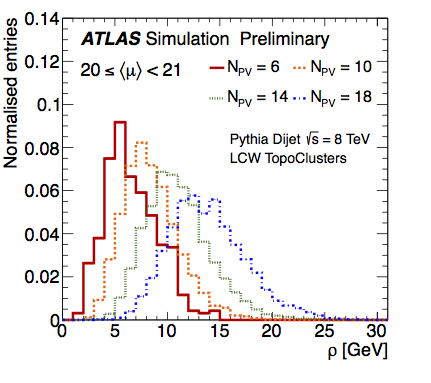
\includegraphics[width=\textwidth]{figures/rho8.png}
	\caption{$\rho$ during Run 1, taken from Ref~~\cite{Malaescu:2048678}}
	\label{fig:rho8}
\end{subfigure} % \hspace{0.2\textwidth}
\begin{subfigure}{0.48\textwidth}
   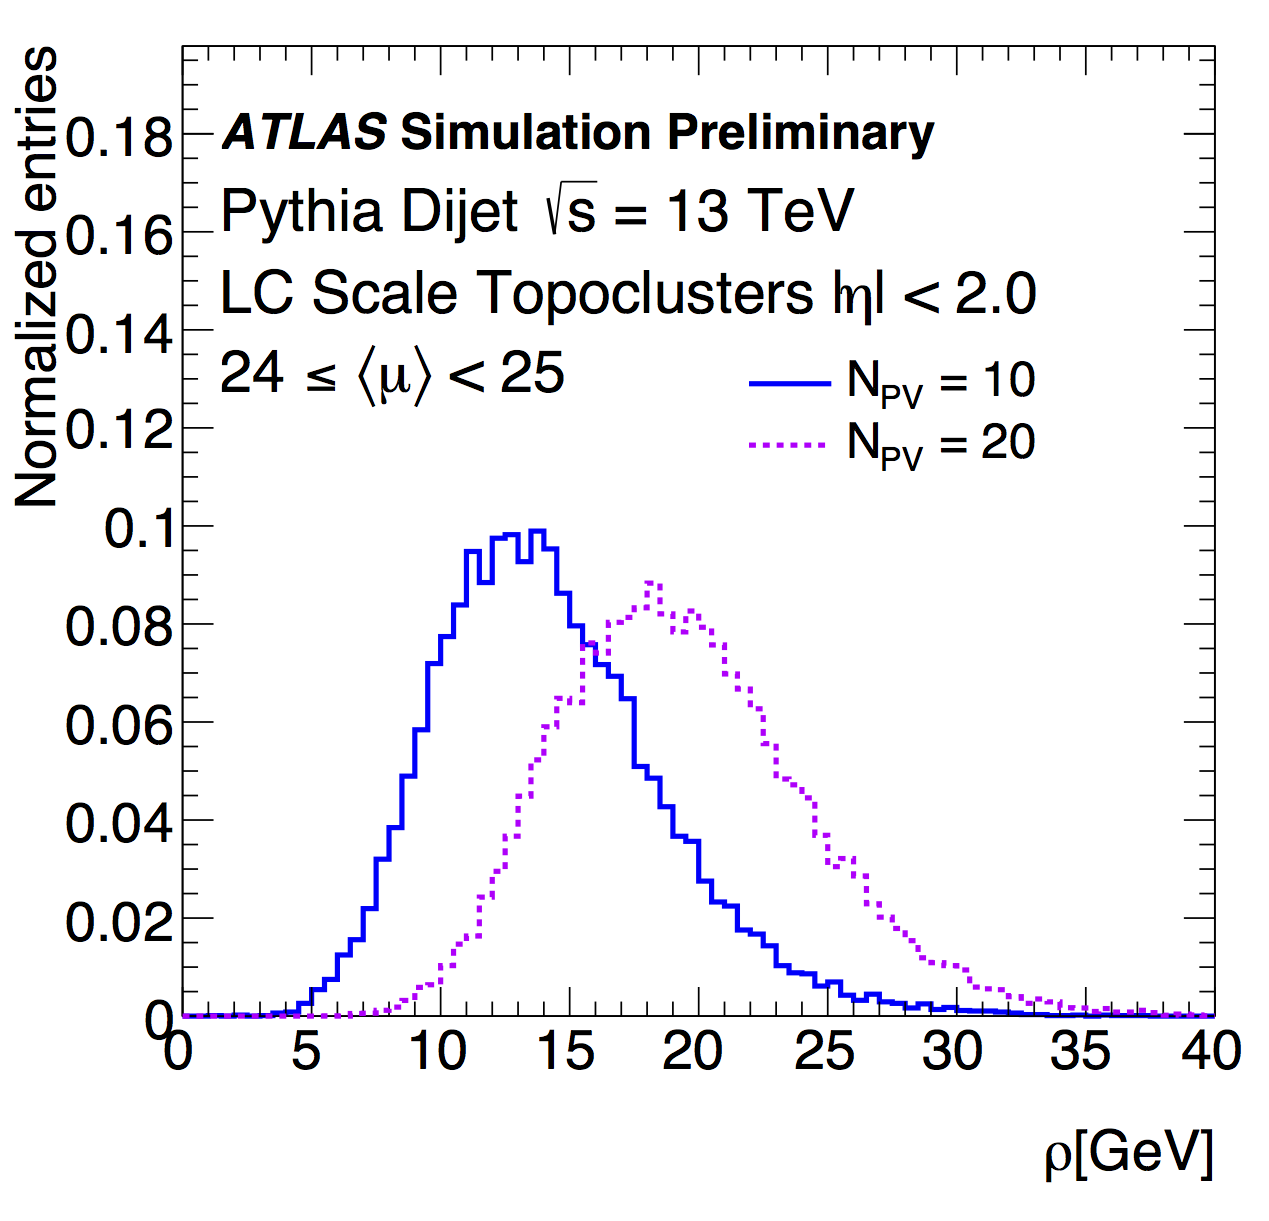
\includegraphics[width=\textwidth]{figures/rho13.png}
	\caption{$\rho$ during Run 2, taken from Ref~\cite{Dandoy:2136864}}
	\label{fig:rho13}
\end{subfigure}
	\caption{Plots showing the pileup density $\rho$, the pileup contribution to jet \pt, 
at several number of vertices $N_{PV}$ for jets reconstructed from LCW topological clusters}
\end{figure}

\subsubsection{Energy Scale and Resolution}
\label{sec:jes}
\par After calibrations schemes described so far have been applied, any remaining jet energy dependence 
on $\eta$ and \pt\ is corrected by comparing the calculated jet energy and the true 
particle jet energy from MC simulation. A jet is matched to a true particle if the true particle 
is within its $\Delta R<0.3$. The jet energy {\it response} (also known as {\it scale}\footnote{These 
terms will be used interchangeably in this text}) $\mathcal{R}$ is defined as the ratio of the 
reconstructed energy $E^{reco}$ to the energy of the true particle jet $E^{true}$. Jet {\it \pt\ 
response} is defined similarly. Jet energy in simulation is finely binned in $E^{true}$ and $\eta_{det}$ bins, 
where $\eta_{det}$ is the pseudo-rapidity in detector coordinates rather than the corrected $\eta$ 
described in Section~\ref{sec:orCorr}. The motivation for $\eta_{det}$ parameterization is that problems may arise from transitioning 
from the barrel to end-cap calorimeters.

\par The jet energy response is measured in bins of $E^{true}$ and $\eta_{det}$. The value in each bin 
is taken as the peak of a gaussian fit for all the values that fall in that bin. 
The energy {\it resolution} is then taken as the standard deviation of the said gaussian 
fit, so it is binned in the same manner as the energy response.  
For each $\eta_{det}$ bin, a calibration function $\mathcal{F}(E^{reco})$ is obtained by a fit of 
$(E^{reco},\mathcal{R})$ values for each $E^{true}$ bin. The corrected jet energy is then 
defined for each $\eta_{det}$ bin as 

\begin{equation}
E^{corr} = E^{reco}/\mathcal{F}(E^{reco})
\end{equation}

where $1/\mathcal{F}(E^{reco})$ is the jet energy scale. A simple approximation, 
$\mathcal{F}(E^{reco}) = \langle E^{reco}/E^{true}\rangle$, was used in both Run I and Run II. 
In this approximation, $\mathcal{F}(E^{reco})$ is the average jet energy response per $\eta_{det}$
bin. Figure~\ref{fig:eResPt} and \ref{fig:eResEta} show the jet energy response for $\pt^{true}$ and $\eta_{det}$ respectively for 
simulated LCW anti-kt jets, with $R=0.4$. The disagreement in the low \pt\ range is caused by non-perfect 
fits which were caused by non-Gaussian effects. 

\begin{figure}[h]
\begin{subfigure}{0.5\textwidth}
   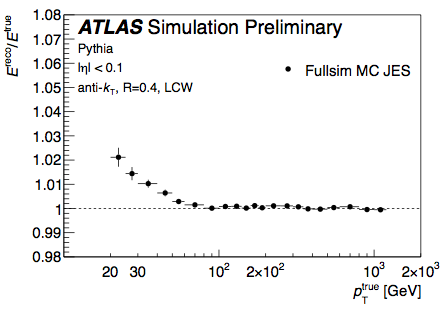
\includegraphics[width=\textwidth]{figures/eResponsePt.png}
	\caption{Jet energy response vs. $\pt^{true}$}
	\label{fig:eResPt}
\end{subfigure} % \hspace{0.1\textwidth}
\begin{subfigure}{0.5\textwidth}
   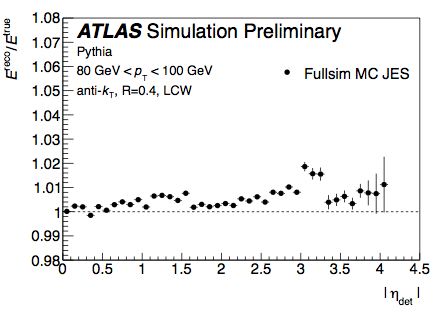
\includegraphics[width=\textwidth]{figures/eResponseEta.png}
	\caption{Jet energy response vs. $\eta_{det}$}
	\label{fig:eResEta}
\end{subfigure}
\caption{Plots showing the jet energy response for simulated LCW jets reconstructed with the 
anti-kt algorithm at R$=0.4$ is plotted against $\pt^{true}$ and $|\eta_{det}|$. 
Taken from Ref~\cite{Malaescu:2048678}}
\end{figure}

\par Studies described in the preceding paragraphs were performed with Monte Carlo simulations 
for several physics processes to evaluate the associated systematic uncertainties. 
These are $Z+$jets, $\gamma+$jets and events with only 2 jets. Jets in the central region were observed 
to have at most 3\% uncertainty in the jet energy scale, and those in the forward regions 
had at most 6\%. The resolution was observed to increase with true \pt\ and with higher pseudorapidity. 
The total uncertainty on the resolution was calculated by varying the Gaussian fits (introduced in this 
section) by $\pm 1\sigma$. This uncertainty was observed to be at most 2\%, varying with the 
true \pt.  

\subsubsection{Jets from pileup}
\par Even after tracks from pileup events that get associated to jets are subtracted with 
the technique described in Section~\ref{sec:ghosts} are subtracted from the jet, jets that originate 
entirely from pileup events are not subtracted from the event. Techniques used to suppress such jets have 
evolved from Run 1 to Run 2. 

\par During Run 1, the Jet Vertex Fraction (JVF)~\cite{TheATLAScollaboration:2013pia} was the main variable used 
to suppress jets from pileup interactions. In an event with multiple reconstructed vertices, 
JVF for a jet was used to determine the likelihood of it originating from each of the 
vertices. Thus, JVF is a function of the jet $\text{jet}_i$ and reconstructed vertex $V_j$ in the 
event. Precisely, it is defined as 

\begin{equation}
\text{JVF}(\text{jet}_i,V_j) = \frac{\sum_m\pt(\text{track}_m^{\text{jet}_i},V_j)}{\sum_n\sum_l\pt(\text{track}_l^{\text{jet}_i},V_n)},
\label{eq:jvf}
\end{equation}  

where $m$ runs over tracks associated with $\text{jet}_i$ and whose origin is $V_j$. $n$ runs over all reconstructed vertices in 
the event and $l$ runs over all tracks whose origin is $V_n$ and associated with
 $\text{jet}_i$. For each of these tracks a $\pt>500~\MeV$ 
requirement is demanded. For jets with no tracks, a value of -1 is assigned to JVF. During Run 1 the vertex of interest was 
the primary vertex, $V_0$. $\text{JVF}(V_0)$ was used as a discriminant for each jet. 
Figure~\ref{fig:jvfPl} shows the $\text{JVF}(V_0)$ distribution for simulation jets from the primary vertex (hard-scatter jets) 
and jets from pileup, for jets with $20<\pt<50~\GeV$ and $|\eta|<2.4$. These jets were reconstructed using the LCW 
scale and the jet energy scale~\ref{sec:jes} (JES) was applied. Pileup jets tend to have low JVF 
because their tracks rarely originate from the primary vertex. Using $\Zmm+$jets events from simulation 
it was observed that pileup jets during Run 1 were suppressed to $2\%$ for jets with $\pt\approx20~\GeV$ 
and even to lower values for jets with higher \pt. 

\begin{figure}[!h]
\centering
   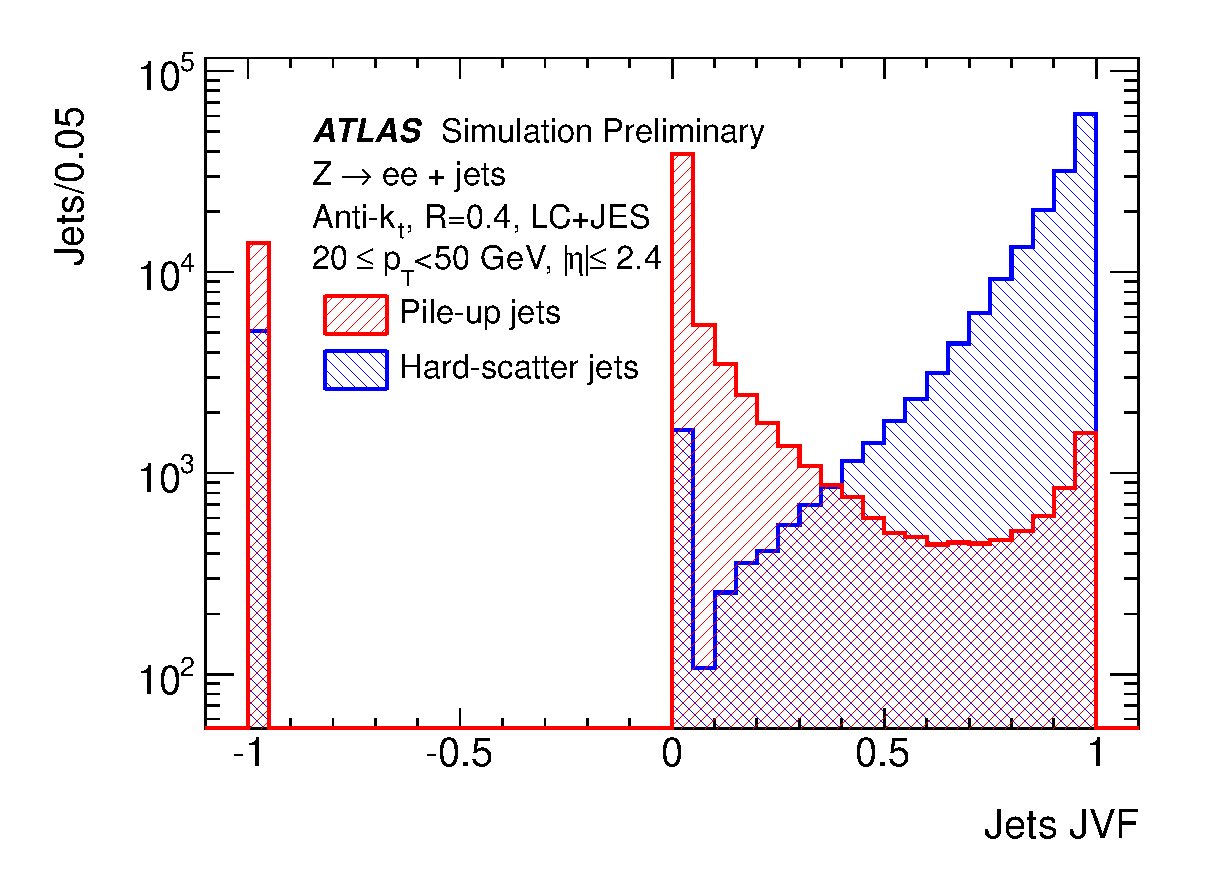
\includegraphics[width=0.8\textwidth]{figures/c_jets_JVF_PUTJ_Simulation_log.eps}
\caption{Plots showing the JVF distributions for pileup jets and jets from the primary vertex (hard-scatter), evaluated 
for the primary vertex. Taken from Ref~\cite{Aad:2015ina}}
	\label{fig:jvfPl}
\end{figure}

\par Although reasonably efficient for low pileup (Run 1) conditions, JVF perfomance is reduced 
for higher pileup conditions. This is because JVF is dependent on the number of reconstructed 
vertices in the event; more tracks in the event makes the denominator in Equation~\ref{eq:jvf} 
large, lowering JVF even for hard-scatter jets. Two variables were defined to correct for this.  
corrJVF corrects for the linear increase of the sum \pt\ of tracks from non-primary vertices
$(\sum_{n\geq 1}\sum_l\pt^{trk_l}(V_n))$ with the number of pileup tracks $(n_{trk}^{PU})$ by scaling 
$n_{trk}^{PU}$ with a correctional factor $k$. corrJVF evaluated at the primary vertex $V_0$ is 
then defined as 

\begin{equation}
\text{corrJVF} = \frac{\sum_m \pt^{trk_m}(V_0)}{\sum_l \pt^{trk_l}(V_0) + \sum_{n\geq 1}\sum_l\pt^{trk_l}(V_n)}
\end{equation}

The second variable used is $R_{\pt}$. It is defined as 

\begin{equation}
R_{\pt} = \frac{\sum_h \pt^{trk_h}(V_0)}{\pt^{\text{jet}}}
\end{equation}

where $h$ runs over all the tracks associated with the jet and originating from the primary vertex, and the denominator 
is the calibrated reconstructed jet \pt\ after subtracting pileup tracks using the ghost tracks technique 
described in the previous section. Figures~\ref{fig:corrJVF} and~\ref{fig:Rpt} show corrJVF and $R_{\pt}$ 
respectively for hard-scatter and pileup jets. In both these variables, a value of -1 is assigned if the 
jet has no associated tracks. For those jets with associated tracks, corrJVF and $R_{\pt}$ are reasonable 
discriminants. 

\begin{figure}[!h]
\begin{subfigure}{0.5\textwidth}
   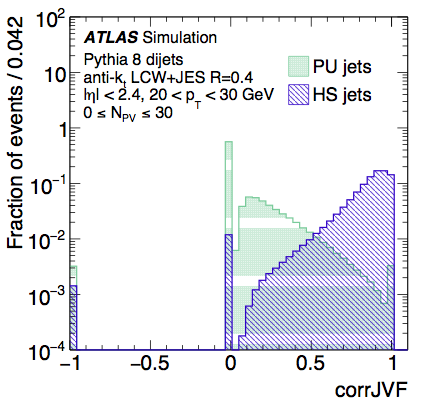
\includegraphics[width=\textwidth]{figures/corrJVF.png}
	\caption{corrJVF}
	\label{fig:corrJVF}
\end{subfigure} % \hspace{0.1\textwidth}
\begin{subfigure}{0.5\textwidth}
   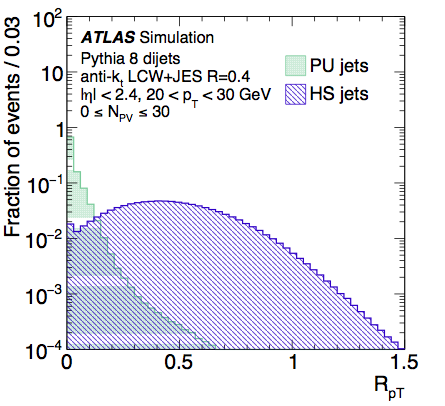
\includegraphics[width=\textwidth]{figures/Rpt.png}
	\caption{$R_{\pt}$}
	\label{fig:Rpt}
\end{subfigure}
\caption{Plots showing distributions of variables used to correct for JVF's dependence on the number of 
reconstructed vertices, and hence number of pileup tracks, in an event. The distributions 
from pileup and hard-scatter jets are overlayed. The simulated jets are reconstructed with the 
LCW scale and the jet energy scale is applied. Taken from Ref~\cite{Aad:2015ina}}
\end{figure}

\par During Run 2 a Jet Vertex Tagger (JVT), which makes use of corrJVF and $R_{\pt}$, 
 is used. corrJVF and $R_{\pt}$ define a 2-dimensional space in which every reconstructed 
jet resides. The k-nearest neighbor (kNN) model~\cite{citeulike:1164920} is used to determine 
the likelihood of a jet to be from hard-scatter (signal) or from pileup (background). This 
model is trained on a sample of signal and background for jets with \pt\ in the range of 
20~\GeV\ and 50~\GeV and $|\eta|<2.4$, where 100 nearest neighbors are used to determine 
the likelihood for a jet to be signal or background. Figure~\ref{fig:jvtROC} shows the fake rate 
from pileup jets versus the efficiency from hard scatter jets from simulation using JVT and other 
discriminants discussed in this section; the JVT curve shows that it is the most optimal of all 
the other pileup suppression techniques. 

\begin{figure}[!h]
\centering
   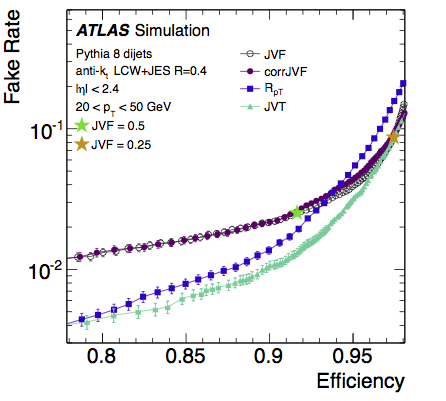
\includegraphics[width=0.8\textwidth]{figures/jvtROC.png}
\caption{Plots showing the fake rate from pileup jets versus efficiency hard scatter jets for JVF, corrJVF, $R_{\pt}$,
and JVT. JVT uses a kNN model in corrJVF-$R_{\pt}$ space where 100 neighbors determine whether a jet is 
from pileup or from hard scatter. Taken from Ref~\cite{Aad:2015ina}}
	\label{fig:jvtROC}
\end{figure}

\par Uncertainties associated with JVF and JVT were calculated by shifting the JVF or JVT selection by 
variations that account for the extent to which the jet correction is mis-modelled for jets 
originating from the primary vertex. These uncertainties vary between 2 and 6\% depending on the 
jet \pt\ and pseudorapidity. 

\subsection{B-Tagging}
\label{sec:bTag}
\par Jets initiated by $b$-quarks are common signatures 
in many processes. For example, in $gg\ra\ttbar$ each 
top quark decays weakly to a bottom quark which then initiates a jet. Several techniques are 
available that tag a jet as $b$-quark initiated. 
$b$-tagging techniques typically exploit the relatively high lifetime 
of the $b$-hadrons, which is of the order of \SI{1.5}{\pico\s}. To put this into perspective, a $b$-hadron 
with $\pt=50~\GeV$ will typically traverse several mm before decaying to $c$-hadrons 
or some other light-flavor hadrons. This section discussed two types of 
$b$-tagging techniques whose details can be found in Ref~\cite{Aad:2015ydr}. 

\par The first technique parameterizes the $b$-hadron lifetime by the impact parameters 
of the tracks in a jet with respect to the primary vertex. The most efficient of algorithms 
that implement this technique is IP3D. It proceeds as follows: For a jet, each track's transverse 
impact parameter with respect to the primary vertex $d_0$ and its longitudinal impact parameter $z_0$
are extracted. A 2-dimensional function of the significance of $d_0$ $(d_0/\sigma(d_0))$, and the 
significance of $z_0$ $(z_0/\sigma(z_0))$ is evaluated and compared to 2-dimensional probability density functions 
for $b$ and light flavor jet hypotheses for each track. These prior probability 
density functions are obtained from Monte Carlo simulations. The ratio of the $b$-jet likelihood to the 
light flavor jet likelihood is taken as the track weight. The weight for the jet is then the 
sum of logarithms of the individual track weights. A simpler version of this algorithm 
is the IP2D, which replaces the 2-dimensional function with a 1-dimensional function of $z_0/\sigma(z_0)$.

\par The second technique constructs a secondary vertex at which the $b$-hadron decays.
The secondary vertex is built by vertices from pairs of tracks with large displacements from the 
primary vertex. These two-track vertices are required to have a fit with a $\chi^2$ lower than a threshold value. 
Additionally, vertices compatible with long lived particles and photon conversions are not considered. 
When building the two-track vertices into the secondary vertex two-track vertices contributing 
the largest $\chi^2$ are removed if the secondary vertex's $\chi^2$ is larger than a threshold value. 
The distance between the primary vertex and the secondary vertex is the discriminant used for 
identifying $b$-jets. One algorithm that implements this technique is called SV1. It uses the 
Log Likelihood Ratio method, where the likelihoods are constructed from two distributions: The 
first is a 2-dimensional distribution of secondary vertex mass versus its energy. The second is 
a 2-dimensional distribution of the number of two-track vertices in the secondary vertex versus 
the $\Delta R$ between the jet axis and the primary-secondary vertices axis.  

\par Another algorithm that constructs a secondary vertex using a slightly different approach is 
called JetFitter. This algorithm runs a trained artificial neural network on 
the jet, looping through each vertex (apart from the primary)
that has at least two tracks. The neural network takes variables that describe the vertex in question 
and has output nodes for either a $b$-vertex or a light flavor vertex. The discriminant to select $b$-jets 
from light flavor jets is taken as the logarithm of the ratio of values in the $b$-node to the value 
in the light flavor node.     

\subsubsection{Performance and Uncertainties}
\par During Run 2 the $b$-tagging algorithms discussed in this section were combined. 
More specifically, in 2015 the combined algorithm was MV2c20 while in 2016 the algorithm used was called MV2c10.
These two algorithms combine IP2D, IP3D, SV1 and JetFitter~\cite{ATL-PHYS-PUB-2016-012}, where 
the variables from each of standalone algorithms were used as inputs to a Boosted Decision Tree (BDT). 
The BDT was trained using jets initiated by $b$-quarks as signal. The background was a composition of 
light-flavor jets, $c$-jets and jets from a hadronic $\tau$ lepton. In MV2c20, 20\% of the background was made up of  
$c$-jets while in MV2c10 10\% of the background was made up of $c$-jets. It was shown that even though MV2c10 
provides similar light-jet rejection to that provided by MV2c20, it provides 40\% more $c$-jet rejection. 
Thus, analyses presented in this text use only MV2c10. Regardless, it is worthwhile to compare 
the performance of MV2c10 against MV2c20.  

\par Figure~\ref{fig:bdtOutput} shows the performance of the MV2c10 BDT output for $b$-, $c$-, and 
light flavor jets in \ttbar\ events. A nominal selection criterion was imposed on the BDT output such that the 
$b$-jet selection efficiency is 77\%. This working point varied with needs. For example, in 
Section~\ref{sec:objCh} the working point was such that the $b$-jet selection efficiency was 70\%. 

\begin{figure}[!h]
\centering
   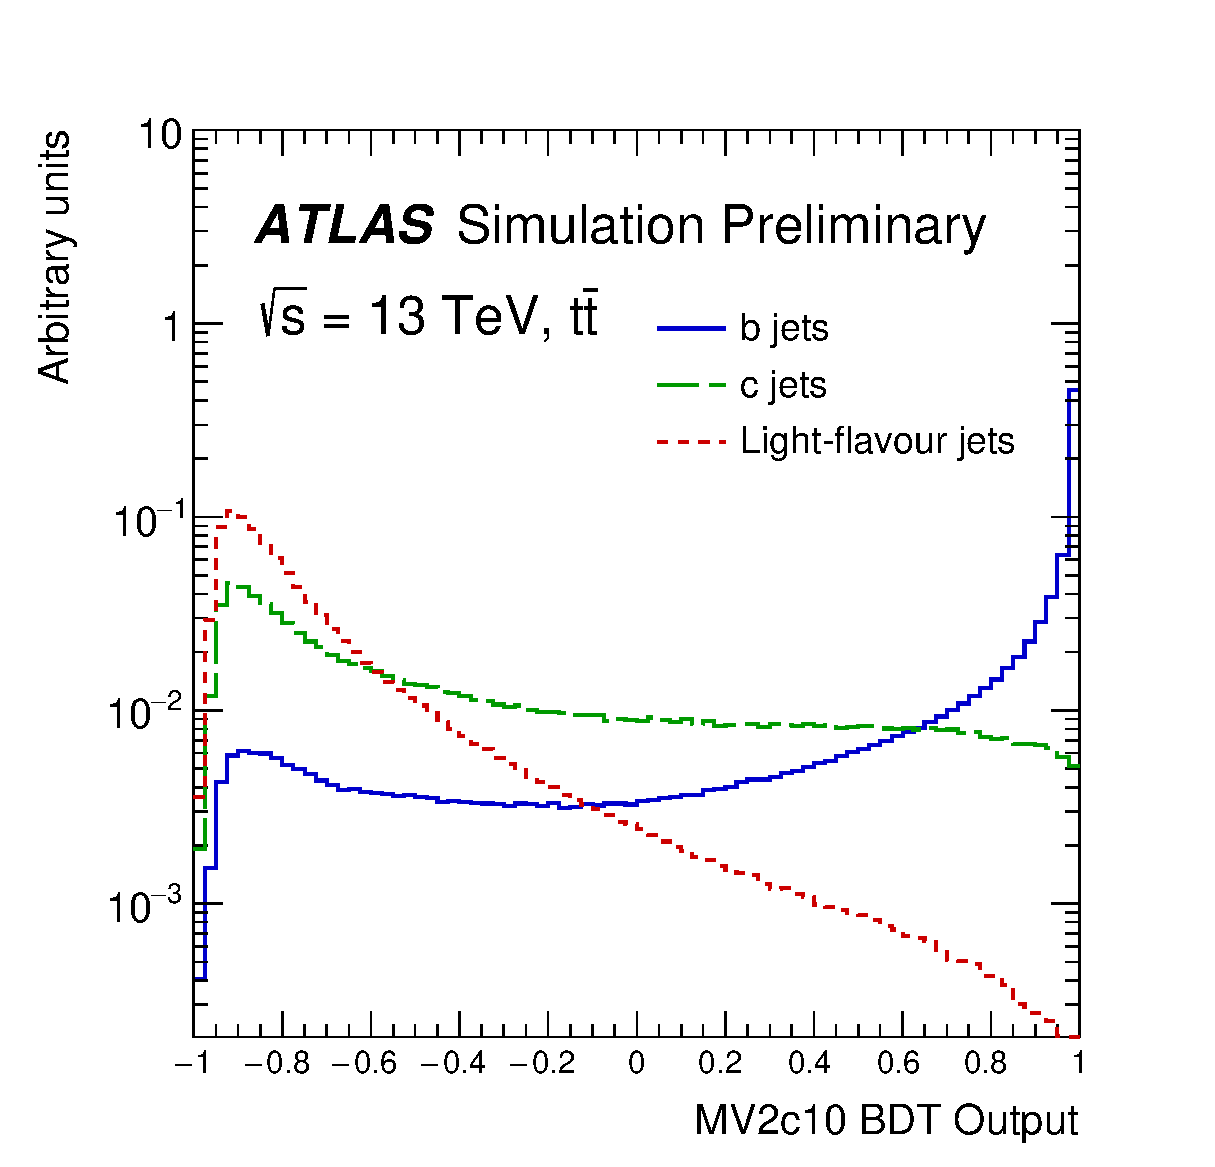
\includegraphics[width=0.8\textwidth]{figures/outputMV2_PRE.eps}
	\caption{Plots showing the MV2c10 BDT output, taken from Ref~~\cite{ATL-PHYS-PUB-2016-012}}
	\label{fig:bdtOutput}
\end{figure}

\par Figure~\ref{fig:effMV2} shows the $b$-jet selection efficiencies, plotted against 
jet \pt, using the BDT outputs from MV2c10 and MV2c20. The working point was 77\% efficiency. 
There is no significant difference between the two algorithms. Figure~\ref{fig:refMV2} shows the 
$c$-jet rejection, plotted against jet \pt, using the BDT outputs from MV2c10 and MV2c20, at a 77\% 
efficiency working point. MV2v10 shows much more improved rejections. That is why it was the 
algorithm of choice in the analysis discussed in Chapter~\ref{chargedH}.   
 
\begin{figure}[!h]
\begin{subfigure}{0.5\textwidth}
   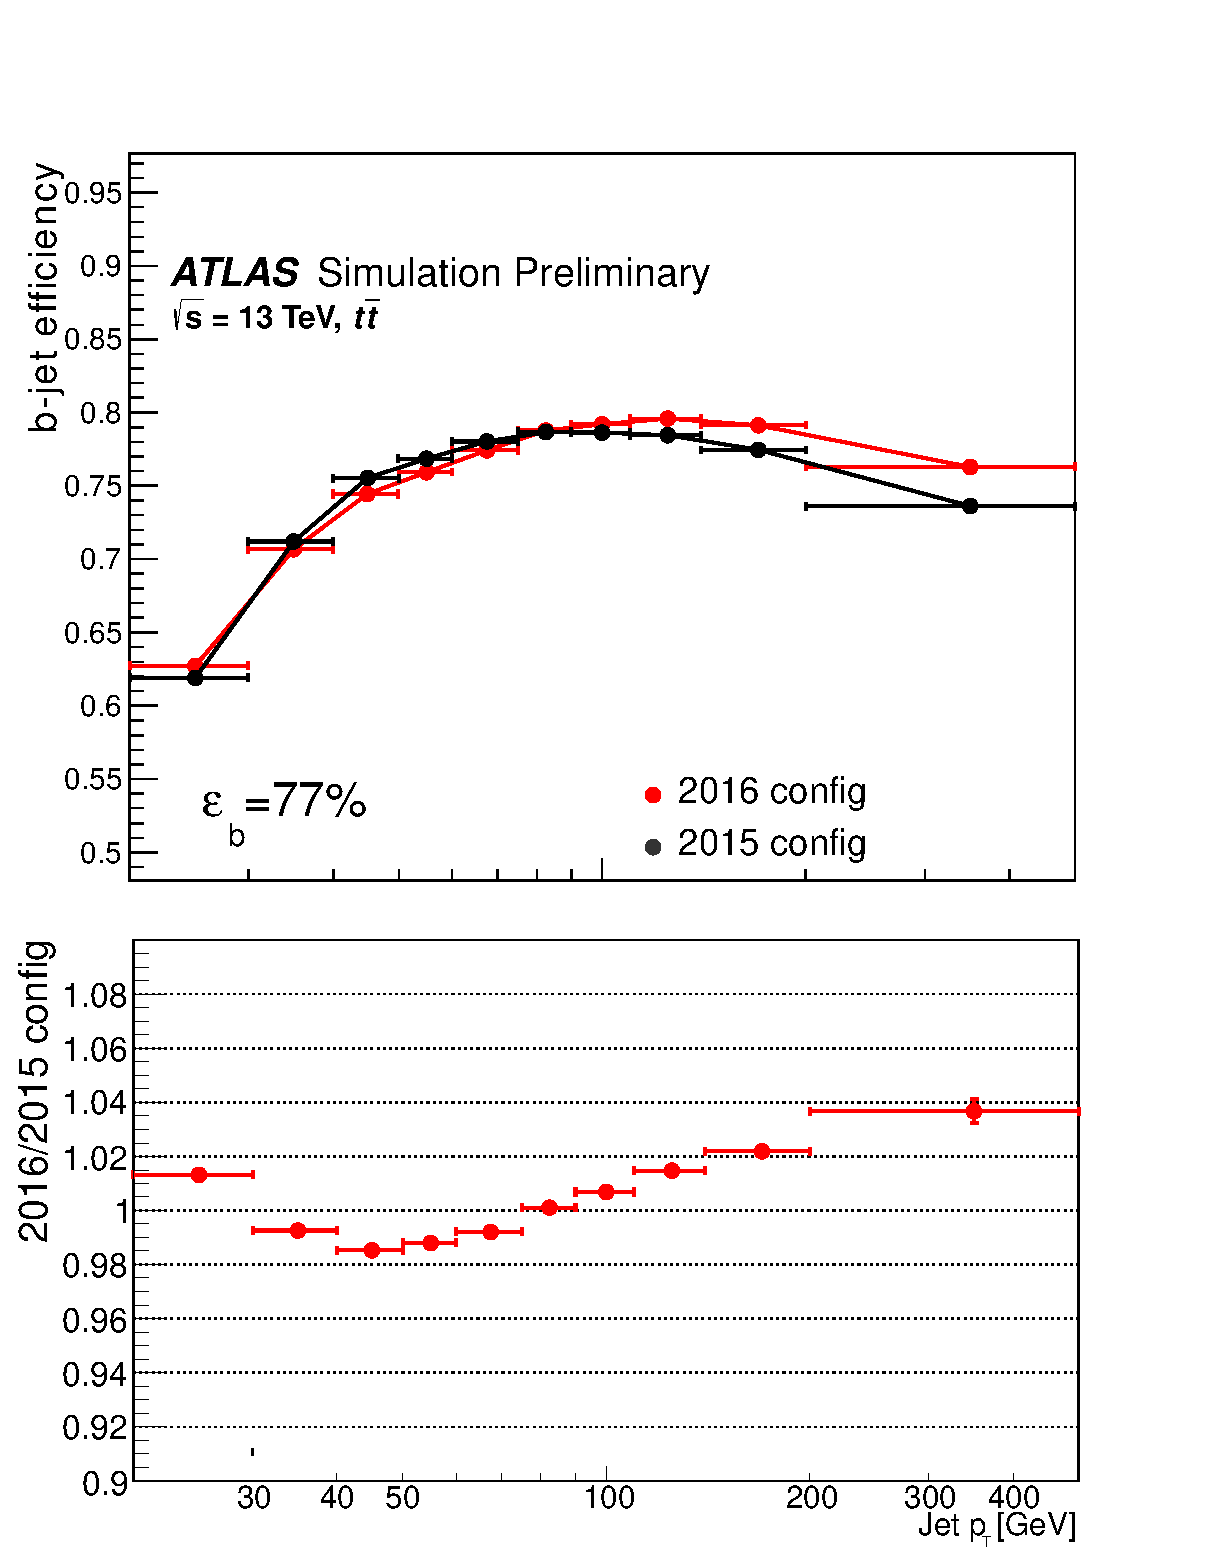
\includegraphics[width=\textwidth]{figures/efficiencyA_PREbis.eps}
	\caption{$b$-jet efficiency}
	\label{fig:effMV2}
\end{subfigure} % \hspace{0.2\textwidth}
\begin{subfigure}{0.5\textwidth}
   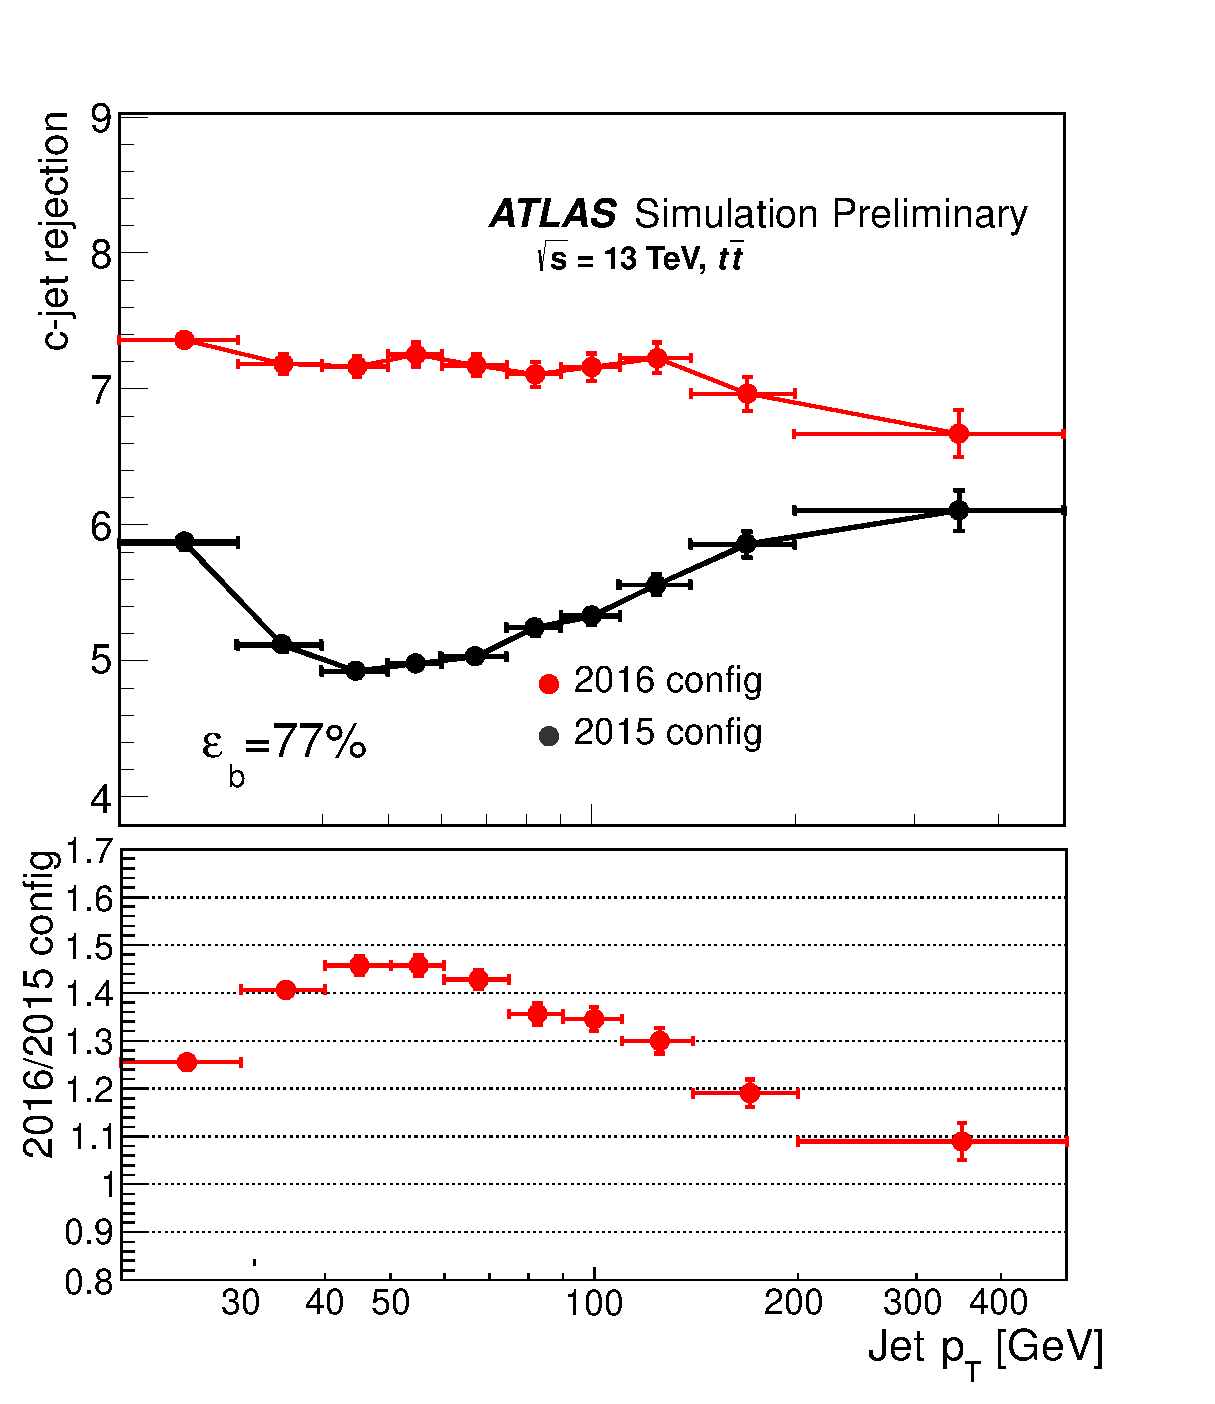
\includegraphics[width=\textwidth]{figures/bc0_modified4BIS_PRE.eps}
	\caption{$c$-jet rejection}
	\label{fig:refMV2}
\end{subfigure}
	\caption{Plots showing the $b$-jet efficiency and $c$-jet rejection parametrized with jet \pt, for the MV2c10 (2016 config)
and the MV2c20 (2015 config) algorithms, at a 77\% $b$-jet selection efficiency working 
point. Taken from Ref~~\cite{ATL-PHYS-PUB-2016-012}}
\end{figure}

\par $b$-tagging efficiencies in Monte Carlo simulations were corrected to match efficiencies obtained in 
regions in data rich in the physics processes modelled by the said Monte Carlo simulations. Uncertainties on the 
$b$-tagging efficiencies were evaluated by shifting the BDT output value by an up and a down value, and 
evaluating the impact on the physics process prediction. More analysis-specific details on this in 
Section~\ref{sec:objCh}. 
